\subsubsection{Package Command}
The command package contains the classes which are a part of the Command design pattern. In our system the Controller and Model parts of the MVC architecture communicate using the Command pattern. The Controller makes function calls to the Model through classes which extend the Command interface. Because the Command pattern serves as an interface between two of the main subsystems, the Command related classes are grouped together in one package. The subsystem is comprised of the Command interface, and any classes extending it, as well as the CommandManager class which maintains a history of the Commands executed.

\paragraph{Detailed Design Diagram}\mbox{}
\begin{figure}[H]
\centering
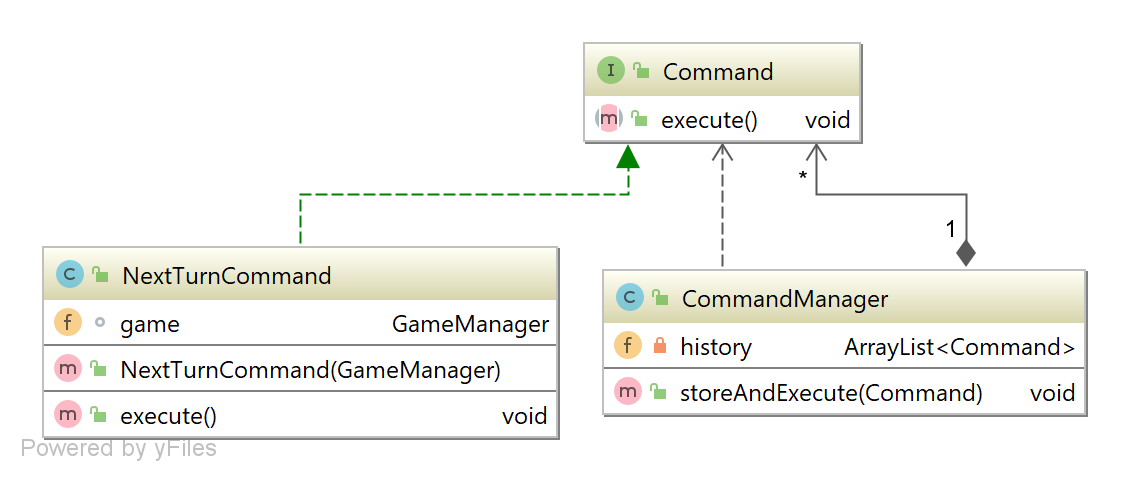
\includegraphics[width=15cm]{Source/Module/Control/Command/Control_Command.png}
\caption{UML Diagram of Package Command in Module Control}
\label{Control.Command}
\end{figure}

\paragraph{Class Command}\mbox{}
\begin{tabularx}{\textwidth}{|c||l|l|l|X|}
    \hline
    \cellcolor{lightgray}Class Name & \multicolumn{4}{X|}{Command}\\
    \hline
    \cellcolor{lightgray}Inherits From & \multicolumn{4}{X|}{None}\\
    \hline
    \cellcolor{lightgray}Description & \multicolumn{4}{p{12cm}|}{Defines interface for commands (Command Pattern)}\\
    \hline\hline
    
    \cellcolor{lightgray}Methods & \cellcolor{lightgray}Visibility & \multicolumn{2}{l|}{\cellcolor{lightgray}Method Name} & \cellcolor{lightgray}Description\\\cline{2-5}
    \cellcolor{lightgray} & Public & \multicolumn{2}{l|}{execute()} & Executes command\\
    \hline
\end{tabularx}
\paragraph{Class CommandManager}\mbox{}
\begin{tabularx}{\textwidth}{|c||l|l|l|X|}
    \hline
    \cellcolor{lightgray}Class Name & \multicolumn{4}{X|}{CommandManager}\\
    \hline
    \cellcolor{lightgray}Inherits From & \multicolumn{4}{X|}{None}\\
    \hline
    \cellcolor{lightgray}Description & \multicolumn{4}{p{12cm}|}{Command manager to execute and store commands and also maintains a history of commands called.}\\
    \hline\hline
    
    \cellcolor{lightgray}Attributes & \cellcolor{lightgray}Visibility & \cellcolor{lightgray}Data type & \cellcolor{lightgray}Name & \cellcolor{lightgray}Description\\\cline{2-5}
    \cellcolor{lightgray} & Private & ArrayList\textlangle{}Command\textrangle{} & history & Object container responsible for containing history of commands\\
    \hline\hline
    
    \cellcolor{lightgray}Methods & \cellcolor{lightgray}Visibility & \multicolumn{2}{l|}{\cellcolor{lightgray}Method Name} & \cellcolor{lightgray}Description\\\cline{2-5}
    \cellcolor{lightgray} & Public & \multicolumn{2}{l|}{storeAndExecute(Command cmd)} & Stores the command in history then uses the execute() method to execute the command\\
    \hline
\end{tabularx}
\paragraph{Class NextTurnCommand}\mbox{}
\begin{tabularx}{\textwidth}{|c||l|l|l|X|}
    \hline
    \cellcolor{lightgray}Class Name & \multicolumn{4}{X|}{NextTurnCommand}\\
    \hline
    \cellcolor{lightgray}Inherits From & \multicolumn{4}{X|}{Command}\\
    \hline
    \cellcolor{lightgray}Description & \multicolumn{4}{p{12cm}|}{A Command to be used by control.GameHandler to tell the GameManager to run the next turn.}\\
    \hline\hline
    
    \cellcolor{lightgray}Attributes & \cellcolor{lightgray}Visibility & \cellcolor{lightgray}Data type & \cellcolor{lightgray}Name & \cellcolor{lightgray}Description\\\cline{2-5}
    \cellcolor{lightgray} & Private & GameManager & game & The part of the model that controls turn flow\\
    \hline\hline
    
    \cellcolor{lightgray}Methods & \cellcolor{lightgray}Visibility & \multicolumn{2}{l|}{\cellcolor{lightgray}Method Name} & \cellcolor{lightgray}Description\\\cline{2-5}
    \cellcolor{lightgray} & Public & \multicolumn{2}{X|}{NextTurnCommand (GameManager game)} & Constructor to set the game to the given input game\\\cline{2-5}
    \cellcolor{lightgray} & Public & \multicolumn{2}{l|}{execute()} & Override execute() command to do next turn.\\
    \hline
\end{tabularx}